\begin{figure*}[t]
    \centering
    \includegraphics[width=0.99\linewidth]{figures/methodology.pdf}
    \caption{Model Architecture Diagram. Top left - illustration of forward generation. Bottom left - illustration of inverse generation. Right - \modelName{} and its four components. We first extract domain-specific triggers via forward generation, then generate passages using inverse generation. Forward generation refines missing events, and we sample $N$ data points per event for downstream training.}
    \label{fig:methodology}
\end{figure*}

\section{Methodology}
\label{sec:methodology}

In this work, we focus on Large Language Model (LLM)-powered synthetic data generation to alleviate the need for domain-specific annotated training data, as zero-shot LLM-based approaches usually struggle in ED in specialized domains \cite{huang-etal-2024-textee}.
By generating a large amount of data instances $D_s = \{(X,Y)\}$, we can train downstream supervised ED models.
Here, we first briefly review prior works on forward generation and backward generation. Next, we introduce our proposed data generation method \modelName.

\subsection{Background}
\label{sec:methodology-background}

We focus on two major paradigms for data generation in our work: forward generation and inverse generation. We describe them briefly below and provide illustrations in Figure~\ref{fig:methodology}.

\paragraph{Forward Generation:}
This is a more straightforward manner of data generation, wherein LLMs are utilized to generate labels $Y'$ on unlabeled data $X \in D_T'$ (i.e. $X \rightarrow Y')$.
This generation is analogous to \textit{weak/distant supervision} (\extracttrain) \cite{mintz-etal-2009-distant, DBLP:journals/corr/abs-2109-09193, DBLP:journals/corr/abs-2106-06168} where noisy/weak labels are assigned to clean sentences and then utilized to train downstream models.
Consequently, the label quality is dependent on the reasoning capability of the LLM.

\paragraph{Inverse Generation:}
Inverse generation is a relatively new data generation paradigm \cite{kumar-etal-2020-data, schick-schutze-2021-generating}.
% with a prominent application in Self-Instruct \cite{wang-etal-2023-self-instruct}.
This paradigm first generates/samples potential labels $Y$ based on the task definition and then generates plausible $X'$ conditioned on the label $Y$ (i.e. $Y \rightarrow X'$).
Recent works like SynthIE \cite{josifoski-etal-2023-exploiting} and STAR \cite{star} have explored the usage of LLM-guided inverse generation for information extraction and event extraction tasks.
Inverse generation provides control over data distribution via prompting, but the data quality is dependent on the LLM's sentence generation capability.

% \subsection{\starName}
% \label{sec:methodology-star}

% \starName{} \cite{star} has been one of the major works which conducted inverse generation for ED.
% We make minor modifications to the original STAR pipeline to make it generalizable across different LLMs.
% There are four major components of this pipeline, described below and illustrated in Figure~\ref{fig:methodology-figure}.

% \paragraph{Target Structure Generation:}
% This component involves utilizing the LLM to generate $T$ trigger words for each event type.
% The LLM is prompted with the task instructions, the event definition, and some examples (in the few-shot setting), and asked to generate some examples of similar trigger words that can be used for the given event type (as illustrated in Figure~\ref{fig:target-structure-generation-prompt}).
% Finally, to create the target structure $Y$, we sample triggers upto 2 event types for each synthetic instance.

% \paragraph{Passage Generation:}
% This component is tasked with generating the passage $X$ corresponding to the structured output $Y$.
% The LLM is prompted with the task instructions, the event definitions, some examples (in the few-shot setting), the sampled target structure $Y$, and asked to generate a passage $X$ which mentions the event types using the triggers in $Y$.
% We provide an illustration of this prompt in Figure~\ref{fig:passage-generation-prompt}.

% \paragraph{Data Refinement and Sampling:}
% To maintain high data quality, we apply an automated rule removing all passages which do not contain the trigger or correcting the trigger annotation if some other form of the trigger word is used.
% Post cleaning, we apply a sampling algorithm to greedily sample $N$ instances per event type to create our final synthetic dataset

\subsection{\modelName}

LLM reasoning has been poor for ED \cite{DBLP:journals/corr/abs-2304-11633, huang-etal-2024-textee}, which makes forward generation vulnerable to noisy label quality.
Since LLMs are pre-trained to generate natural sentences, their generation capabilities are stronger, which supports inverse generation.
However, owing to the lack of any domain-specific information, inverse generation can synthesize highly diverse sentences, leading to a domain drift.
Merely specifying the domain in the prompt is not sufficient (shown in \S~\ref{sec:appendix-analysis-star-domain}).
Furthermore, inverse generation sentences can mention additional events which remain unannotated introducing noise in the data.

To this end, we propose \textbf{F}orward-\textbf{I}nverse \textbf{G}eneration (\modelName), a hybrid approach that infuses forward generation reasoning into the base pipeline of inverse generation to ensure closer alignment to the target domain while improving the quality of the annotated labels.
To procure domain-specific cues, we assume access to an unlabeled target domain data $D_T'$ (similar to forward generation).
We provide our architectural diagram in Figure~\ref{fig:methodology} and explain each component of our pipeline below.

\paragraph{Target Structure Extraction:}
Similar to inverse generation, we first create potential triggers (i.e. labels) for each event type.
However, generation from scratch can lead to very divergent set of triggers.
For example, an ``Attack" event can refer to a war in the news, cyberattacks in the cybersecurity domain, diseases in epidemiology, or criticism in economics.
Naturally, each scenario would assume different triggers, which inverse generation struggles to generate even when provided with clear event definitions (actual examples in \S~\ref{sec:qual-analysis}).

Instead, we generate potential triggers per event type by utilizing an LLM to extract triggers using a forward generation over the unlabeled data $D_T'$.
To ensure highly precise extraction of triggers, we develop a two-stage prompt setup.
The first stage is tasked to identify and filter possible event types mentioned in the text based on the task instructions and event definitions.
The second stage aims to find the most appropriate trigger word from the unlabeled sentence for each filtered event type.
We illustrate this setup in \S~\ref{sec:appendix-exgen-prompts}.

After extraction, we aggregate and sort the triggers for each event type at the corpus level and filter out the top $t$ triggers for each event type as the set of clean triggers.
This filtering helps remove many noisy triggers introduced in the forward generation.
Finally, we create target structures $Y$ by sampling 1-2 event types per instance and sampling triggers from the clean trigger set for each sampled event type.
We ensure uniform sampling of event types and triggers to avoid unbalanced label distribution.
Overall, such forward generation-based trigger extraction ensures the distillation of domain-specific knowledge in the target structures.

\paragraph{Passage Generation:}
This component is the core of inverse generation and is tasked with generating passages corresponding to the constraints of the sampled target structure.
Specifically, the LLM is prompted with the task instructions, the event definitions, the sampled target structure $Y$, and asked to generate a passage $X'$ which mentions the event types using the triggers in $Y$.
We illustrate this prompt in Figure~\ref{fig:dg_prompt}.
The key to generating better target data aligned passages lies in the presence of the target data aligned target structure $Y$ (shown via examples in \S~\ref{sec:qual-analysis}).

% To further align the generated passages to the target domain, we propose to utilize the unlabeled data $D_T'$ to fine-tune the LLM via continual pretraining loss.
% This fine-tuned LLM is then used to generate passages.
% Since fine-tuning large LLMs is infeasible, we provide an ablation analysis for fine-tuning on a smaller LLM in \S~\ref{sec:analysis-target-sft}.

\paragraph{Data Refinement and Sampling:}
While passage generation ensures the target structure events are mentioned in the passage, the passage could still have other unknown events which can lead to under-annotated $(X',Y)$ data instances.
We provide an illustration in Figure~\ref{fig:missing-annotation} with the target trigger \textit{positive}, but the generated sentence also has a missing mention of \textit{symptom} event triggered by \textit{got}.
To account for such missing annotations, we utilize forward generation to identify all possible event mentions in the generated passage.
We remove duplicates and add the new event mentions to create a more complete target structure $Y_f$.

\definecolor{eventBlue}{RGB}{41,121,255}    % Generated events
\definecolor{eventRed}{RGB}{255,99,71}      % Missed events
\usetikzlibrary{shapes,arrows,positioning,fit,calc,shadows}
\begin{figure}
    \centering
    \resizebox{0.85\columnwidth}{!}{
    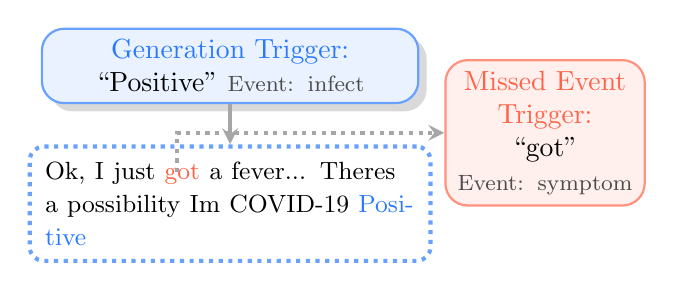
\begin{tikzpicture}[
        % Node styles
        base/.style={
            draw,
            rounded corners=8pt,
            inner sep=4.0pt,
            align=center,
            thick
        },
        generated/.style={
            base,
            text width=4.5cm,
            fill=eventBlue!10,
            draw=eventBlue!70,
            drop shadow={shadow xshift=3pt, shadow yshift=-3pt, opacity=0.3}
        },
        missing/.style={
            base,
            text width=2.25cm,
            fill=eventRed!10,
            draw=eventRed!70
        },
        % Arrow styles
        arrow/.style={
            ->,
            >=stealth,
            line width=1.5pt,
            gray!70
        },
        arrow_missing/.style={
            arrow,
            dotted
        },
        % Text box style
        textbox/.style={
            draw=eventBlue!70,
            dotted,
            line width=1.5pt,
            rounded corners=5pt,
            inner sep=2pt
        }
    ]
        
        % Missing event annotation
        \node[missing] (miss) at (4.0,0.9) {
            \textcolor{eventRed}{Missed Event Trigger:}\\[0pt]
            ``got'' \\
            \footnotesize{\textcolor{black!70}{Event: symptom}}
        };
        
        % Generated event
        \node[generated] (gen) at (0, 1.75) {
            \textcolor{eventBlue}{Generation Trigger:}\\[0pt]
            ``Positive'' \footnotesize{\textcolor{black!70}{Event: infect}}
        };
        
        % Main text
        \node[align=left, text width=4.70cm] (text) at (0,0) {
            \small{Ok, I just \textcolor{eventRed}{got} a fever... Theres a possibility Im COVID-19 \textcolor{eventBlue}{Positive}}
        };
        \node[textbox, fit=(text)] {};
        
        % Arrows
        \draw[arrow] (gen.south) -- ($(text.north)+(0.0,0.1)$);
        \draw[arrow_missing] ($(text.west)+(1.80,0.4)$) |- (miss.west);
        
    \end{tikzpicture}
    }
    \caption{Illustration of how inverse generation can produce unannotated event mentions. Blue box = target event mention, red box = unannotated event mention.}
    \label{fig:missing-annotation}
\end{figure}

To further improve data quality, we apply an automated rule to remove passages that do not mention the target trigger.
Additionally, we standardize trigger annotations by correcting variations in trigger word forms.
Finally, we apply a greedy sampling algorithm to sample $N$ instances $(X', Y_f)$ per event type to create our final synthetic dataset $D_s$.

\paragraph{Downstream Model Training:}
The final component utilizes the generated synthetic data $D_s$ to train downstream ED models in a supervised manner.
The trained ED models are then used for inferring on the test set and for eventual evaluation.

